% !Tex program = pdflatex

\documentclass[UTF8]{ctexart}
\ctexset{section={format={\Large\bfseries}}}
\usepackage{amsmath}
\usepackage{array}
\usepackage{ulem}
\usepackage{graphicx}
\usepackage{booktabs}
\usepackage{listings}
\usepackage{xcolor}
\usepackage{geometry}
\usepackage{multirow}
\usepackage{subfig}
\usepackage{float}
\usepackage{multicol}
\usepackage{multirow}
\usepackage{pgfplots}
\pgfplotsset{compat=1.18}
\usepackage{diagbox}
\usepackage{indentfirst}
\setlength{\parindent}{2em}
\setlength{\parskip}{0.6em}
\setlength{\headheight}{13pt}
\usepackage{makecell}
\geometry{papersize={21cm,29.7cm}}
\geometry{left=2.54cm,right=2.54cm,top=3.18cm,bottom=3.18cm}
\usepackage{fancyhdr}
\pagestyle{fancy}
\lhead{\today}
\chead{}
\rhead{2023012274}
\lfoot{清华大学}
\cfoot{\thepage}
\rfoot{模式识别与机器学习}
\renewcommand{\headrulewidth}{0.4pt}
\renewcommand{\headwidth}{\textwidth}
\renewcommand{\footrulewidth}{0pt}
\usepackage{bm}
% listings style for code snippets
\lstset{
    backgroundcolor=\color{white},
    basicstyle=\ttfamily\small,
    breaklines=true,
    framesep=4pt,
    frame=single,
    rulecolor=\color{gray!40},
    keywordstyle=\color{blue},
    commentstyle=\color{gray!60}\itshape,
    showstringspaces=false,
}

\begin{document}
\begin{titlepage}
     \begin{center}
        \quad \\
        \quad \\
        \quad \\
        \quad \\
        \quad \\
        \quad \\
        \quad \\
        \quad \\ 
        \quad \\ 
        {\kaishu \fontsize{30}{15}\selectfont 《模式识别与机器学习》}\\
        \quad \\
        \quad \\
        {\kaishu \fontsize{30}{15}\selectfont 实验:决策树分类}\\

        \end{center}
        \vskip 8cm

        \begin{center}
        \begin{large}
        \begin{tabular}{cc}
        院\qquad 系:& ~~~~~~~~自动化系~~~~~~~~      \\
        \cline{2-2}\\
        班\qquad 级:& 自31班   \\
        \cline{2-2}\\
        学生姓名:& 苟左    \\
        \cline{2-2}\\
        学\qquad 号:&2023012274   \\
        \cline{2-2}
          \end{tabular}
        \end{large}
      \end{center}

\end{titlepage}
\newpage

\section{实验目的}
\begin{enumerate}
    \item 理解决策树的基本原理及其变种算法(ID3、C4.5、CART)的特点与差异。
    \item 掌握信息熵、信息增益、信息增益率、基尼指数等特征选择准则的计算方法。
    \item 实现预剪枝和后剪枝算法,理解剪枝在决策树中的作用与意义。
    \item 在不同规模数据集上比较决策树算法的性能,分析过拟合现象及其缓解方法。
\end{enumerate}

\section{实验任务与方法}

\subsection{数据集}
本实验使用两个数据集:
\begin{enumerate}
    \item \textbf{Melon 数据集}:迷你西瓜数据集,包含 17 个训练样本和 7 个测试样本,4 个特征(纹理、根蒂、色泽、脐部),2 个类别(好瓜/坏瓜)。该数据集用于算法验证和可视化。
    
    \item \textbf{CelebA 子集}:人脸属性数据集,包含 250 个训练样本和 50 个测试样本,40 个二值属性特征(如性别、头发颜色、五官特征等),10 个类别(不同人物 ID)。该数据集用于评估算法在实际问题上的性能。
\end{enumerate}

\subsection{决策树算法}

\subsubsection{ID3 算法}
ID3(Iterative Dichotomiser 3)使用\textbf{信息增益}作为特征选择准则:

\begin{equation}
\text{Gain}(D, a) = \text{Ent}(D) - \sum_{v=1}^{V}\frac{|D^v|}{|D|}\text{Ent}(D^v)
\end{equation}

\noindent 其中信息熵定义为:
\begin{equation}
\text{Ent}(D) = -\sum_{k=1}^{|\mathcal{Y}|}p_k\log_2 p_k
\end{equation}

\noindent ID3 选择信息增益最大的特征进行划分。

\subsubsection{C4.5 算法}
C4.5 算法使用\textbf{信息增益率}作为特征选择准则,解决了 ID3 偏好取值多的特征的问题:

\begin{equation}
\text{Gain\_ratio}(D, a) = \frac{\text{Gain}(D, a)}{\text{IV}(a)}
\end{equation}

\noindent 其中固有值(Intrinsic Value)定义为:
\begin{equation}
\text{IV}(a) = -\sum_{v=1}^{V}\frac{|D^v|}{|D|}\log_2\frac{|D^v|}{|D|}
\end{equation}

\subsubsection{CART 算法}
CART(Classification And Regression Tree)使用\textbf{基尼指数}作为特征选择准则:

\begin{equation}
\text{Gini}(D) = 1 - \sum_{k=1}^{|\mathcal{Y}|}p_k^2
\end{equation}

\begin{equation}
\text{Gini\_index}(D, a) = \sum_{v=1}^{V}\frac{|D^v|}{|D|}\text{Gini}(D^v)
\end{equation}

\noindent CART 选择基尼指数最小的特征进行划分。

\subsection{剪枝算法}

\subsubsection{预剪枝(Pre-pruning)}
预剪枝在决策树构建过程中,每次划分前先评估划分是否能提升泛化性能:
\begin{enumerate}
    \item 计算划分前在验证集上的准确率 $\text{Acc}_{\text{before}}$
    \item 计算划分后在验证集上的准确率 $\text{Acc}_{\text{after}}$
    \item 若 $\text{Acc}_{\text{after}} \leq \text{Acc}_{\text{before}}$,则禁止划分,将当前节点标记为叶节点
\end{enumerate}

\noindent \textbf{优点}:降低过拟合风险,减少训练和测试时间。

\noindent \textbf{缺点}:可能欠拟合,因为某些划分虽然当前无法提升性能,但后续划分可能有益。

\subsubsection{后剪枝(Post-pruning)}
后剪枝在决策树完全生长后,自底向上地考察每个非叶节点:
\begin{enumerate}
    \item 计算子树在验证集上的准确率 $\text{Acc}_{\text{tree}}$
    \item 将子树替换为叶节点,计算叶节点在验证集上的准确率 $\text{Acc}_{\text{leaf}}$
    \item 若 $\text{Acc}_{\text{leaf}} > \text{Acc}_{\text{tree}}$,则执行剪枝,用叶节点替换子树
\end{enumerate}

\noindent \textbf{优点}:泛化性能通常优于预剪枝,因为基于完整的树结构做决策。

\noindent \textbf{缺点}:训练时间较长,需要先生成完整决策树。

\section{实验实现与代码片段}

\subsection{信息熵计算(tree.py)}
\begin{lstlisting}[language=Python, caption=信息熵计算]
def cal_entropy(dataset):
    numEntries = len(dataset)
    labelCounts = {}
    
    # 统计每个类别的样本数量
    for featVec in dataset:
        currentLabel = featVec[-1]
        if currentLabel not in labelCounts:
            labelCounts[currentLabel] = 0
        labelCounts[currentLabel] += 1
    
    entropy = 0.0
    # 计算信息熵: Ent(D) = -sum(p_k * log2(p_k))
    for count in labelCounts.values():
        prob = count / numEntries
        entropy += -prob * log(prob, 2)
    
    return entropy
\end{lstlisting}

\subsection{ID3 特征选择(tree.py)}
\begin{lstlisting}[language=Python, caption=ID3 算法的特征选择]
def ID3_chooseBestFeatureToSplit(dataset):
    numFeatures = len(dataset[0]) - 1
    baseEnt = cal_entropy(dataset)
    bestInfoGain = 0.0
    bestFeature = -1
    
    for i in range(numFeatures):
        featList = [example[i] for example in dataset]
        uniqueVals = set(featList)
        
        newEnt = 0.0
        for value in uniqueVals:
            subdataset = splitdataset(dataset, i, value)
            prob = len(subdataset) / len(dataset)
            newEnt += prob * cal_entropy(subdataset)
        
        infoGain = baseEnt - newEnt
        
        if infoGain >= bestInfoGain:
            bestInfoGain = infoGain
            bestFeature = i
    
    return bestFeature
\end{lstlisting}

\subsection{C4.5 特征选择(tree.py)}
\begin{lstlisting}[language=Python, caption=C4.5 算法的特征选择]
def C45_chooseBestFeatureToSplit(dataset):
    numFeatures = len(dataset[0]) - 1
    baseEnt = cal_entropy(dataset)
    bestInfoGainRatio = 0.0
    bestFeature = -1
    
    for i in range(numFeatures):
        featList = [example[i] for example in dataset]
        uniqueVals = set(featList)
        
        newEnt = 0.0
        IV = 0.0
        
        for value in uniqueVals:
            subdataset = splitdataset(dataset, i, value)
            prob = len(subdataset) / len(dataset)
            newEnt += prob * cal_entropy(subdataset)
            IV += -prob * log(prob, 2) if prob != 0 else 0
        
        infoGain = baseEnt - newEnt
        # 避免除零错误
        if IV == 0:
            infoGainRatio = 0.0
        else:
            infoGainRatio = infoGain / IV  # 信息增益率
        
        if infoGainRatio >= bestInfoGainRatio:
            bestInfoGainRatio = infoGainRatio
            bestFeature = i
    
    return bestFeature
\end{lstlisting}

\subsection{CART 特征选择(tree.py)}
\begin{lstlisting}[language=Python, caption=CART 算法的特征选择]
def CART_chooseBestFeatureToSplit(dataset):
    numFeatures = len(dataset[0]) - 1
    bestGini = float('inf')
    bestFeature = -1
    
    for i in range(numFeatures):
        featList = [example[i] for example in dataset]
        uniqueVals = set(featList)
        gini = 0.0
        
        for value in uniqueVals:
            subdataset = splitdataset(dataset, i, value)
            classCounts = Counter([example[-1] for example in subdataset])
            
            # 计算子数据集的基尼值
            prob = len(subdataset) / len(dataset)
            sub_gini = 1.0
            for count in classCounts.values():
                sub_prob = count / len(subdataset)
                sub_gini -= sub_prob ** 2
            
            gini += prob * sub_gini
        
        if gini <= bestGini:
            bestGini = gini
            bestFeature = i
    
    return bestFeature
\end{lstlisting}

\subsection{预剪枝实现(tree.py)}
\begin{lstlisting}[language=Python, caption=预剪枝关键代码]
if pre_pruning:
    # 计算划分前在测试集上的分类准确率
    ans = [example[-1] for example in test_dataset]
    result_counter = Counter([example[-1] for example in dataset])
    pre_split_output = result_counter.most_common(1)[0][0]
    pre_split_acc = cal_acc([pre_split_output] * len(test_dataset), ans)
    
    # 计算划分后准确率
    outputs = []
    ans = []
    for value in sorted(uniqueVals):
        cut_testset = splitdataset(test_dataset, bestFeat, value)
        cut_dataset = splitdataset(dataset, bestFeat, value)
        
        for vec in cut_testset:
            ans.append(vec[-1])
        
        if len(cut_dataset) == 0:
            leaf_output = majorityCnt(classList)
        else:
            leaf_output = majorityCnt([example[-1] for example in cut_dataset])
        
        outputs += [leaf_output] * len(cut_testset)
    
    post_split_acc = cal_acc(outputs, ans)
    
    # 如果划分后准确率没有提升,则禁止划分
    if post_split_acc <= pre_split_acc:
        return pre_split_output
\end{lstlisting}

\subsection{后剪枝实现(tree.py)}
\begin{lstlisting}[language=Python, caption=后剪枝关键代码]
if post_pruning and len(test_dataset) != 0:
    # 计算后剪枝前的准确率(保留子树)
    tree_output = classifytest(DecisionTree, featLabels, test_dataset)
    ans = [example[-1] for example in test_dataset]
    tree_acc = cal_acc(tree_output, ans)
    
    # 计算后剪枝后的准确率(替换为叶节点)
    result_counter = Counter([example[-1] for example in dataset])
    post_prune_output = result_counter.most_common(1)[0][0]
    post_prune_acc = cal_acc([post_prune_output] * len(test_dataset), ans)
    
    # 如果剪枝后准确率更高,则执行剪枝
    if post_prune_acc > tree_acc:
        return post_prune_output
\end{lstlisting}

\section{实验结果}

\subsection{Melon 数据集实验}

Melon 数据集初始信息熵 $\text{Ent}(D) = 1.0$(正负样本平衡)。表 \ref{tab:melon_results} 展示了 ID3 算法在不同剪枝策略下的性能对比。

\begin{table}[H]
    \centering
    \caption{Melon 数据集上 ID3 算法的实验结果}
    \label{tab:melon_results}
    \begin{tabular}{lccccc}
    \toprule
    \textbf{剪枝策略} & \textbf{树深度} & \textbf{测试准确率} & \textbf{正确/总数} & \textbf{树结构复杂度} \\
    \midrule
    不剪枝 & 5 & 42.86\% & 3/7 & 高(过拟合) \\
    预剪枝 & 1 & \textbf{71.43\%} & 5/7 & 低(最简单) \\
    后剪枝 & 3 & \textbf{71.43\%} & 5/7 & 中等 \\
    \bottomrule
    \end{tabular}
\end{table}

\noindent \textbf{结论}:不剪枝导致严重过拟合(42.86\%),剪枝将准确率提升至 71.43\%(提升 67\%)。预剪枝树最简单(深度 1),后剪枝保留更多结构(深度 3)但准确率相同。首选特征为\textbf{脐部}和\textbf{色泽}(信息增益均为 0.275)。图 \ref{fig:melon_trees} 展示了三种策略的决策树结构对比。

\begin{figure}[H]
    \centering
    \subfloat[不剪枝(过拟合)]{
        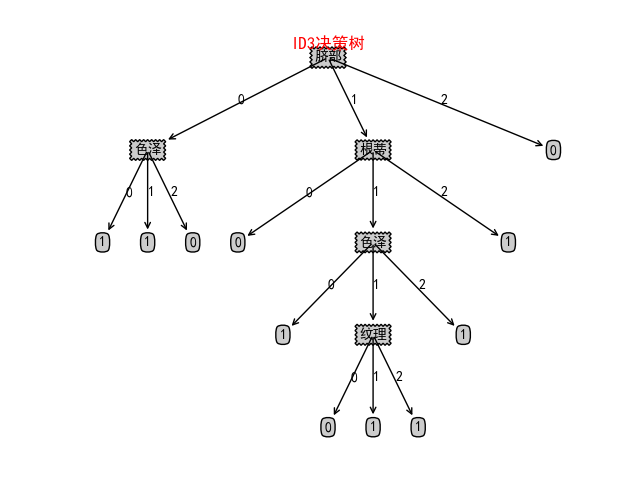
\includegraphics[width=0.3\textwidth]{../figs/melon_id3_full.png}
    }
    \hfill
    \subfloat[预剪枝(最简)]{
        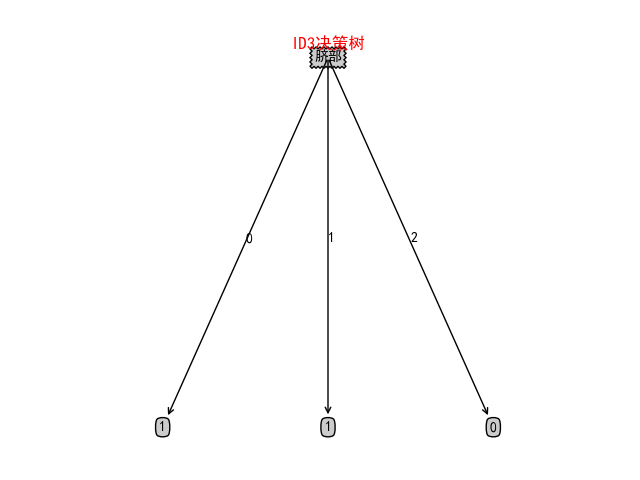
\includegraphics[width=0.3\textwidth]{../figs/melon_id3_pre.png}
    }
    \hfill
    \subfloat[后剪枝(平衡)]{
        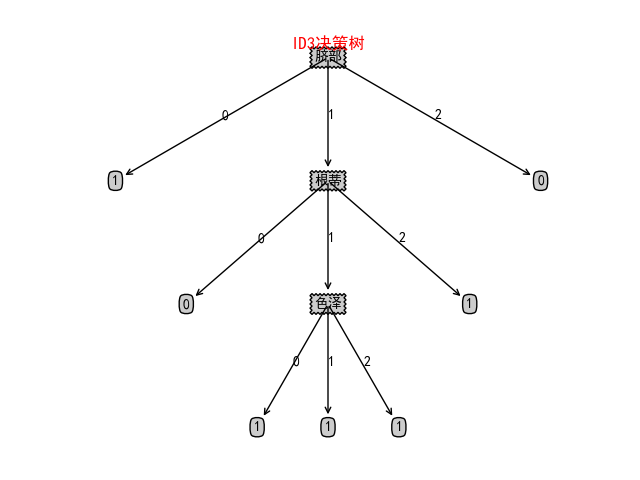
\includegraphics[width=0.3\textwidth]{../figs/melon_id3_post.png}
    }
    \caption{Melon 数据集 ID3 决策树结构对比}
    \label{fig:melon_trees}
\end{figure}

\subsection{CelebA 数据集实验}

CelebA 子集的初始信息熵为 $\text{Ent}(D) = 3.322$,显著高于 Melon 数据集,反映了 10 分类问题的高复杂度。表 \ref{tab:celeba_results} 总结了在 CelebA 数据集上的实验结果。

\begin{table}[H]
    \centering
    \caption{CelebA 数据集上不同算法的实验结果}
    \label{tab:celeba_results}
    \begin{tabular}{lcccc}
    \toprule
    \textbf{算法} & \textbf{剪枝策略} & \textbf{测试准确率} & \textbf{正确/总数} & \textbf{首选特征} \\
    \midrule
    ID3 & 预剪枝 & 76\% & 38/50 & Male(信息增益 0.896) \\
    ID3 & 后剪枝 & \textbf{86\%} & 43/50 & Male(信息增益 0.896) \\
    \midrule
    C4.5 & 预剪枝 & 68\% & 34/50 & Big\_Nose(增益率 0.589) \\
    C4.5 & 后剪枝 & 84\% & 42/50 & Big\_Nose(增益率 0.589) \\
    \midrule
    CART & 预剪枝 & 76\% & 38/50 & Male(基尼指数 0.838) \\
    CART & 后剪枝 & 84\% & 42/50 & Male(基尼指数 0.838) \\
    \bottomrule
    \end{tabular}
\end{table}

\subsubsection{ID3 算法在 CelebA 上的表现}

ID3 算法首选特征为 \textbf{Male}(性别),信息增益高达 \textbf{0.896},远超其他特征。\textbf{预剪枝}达到 76\% 准确率,\textbf{后剪枝}达到 \textbf{86\%} 准确率(最佳性能)。图 \ref{fig:celeba_id3} 展示了 ID3 在不同剪枝策略下的决策树结构。

\begin{figure}[H]
    \centering
    \subfloat[ID3 预剪枝]{
        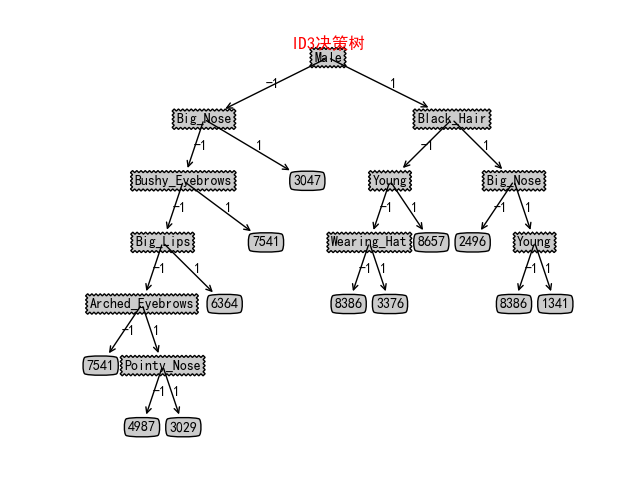
\includegraphics[width=0.45\textwidth]{../figs/celeba_id3_pre.png}
    }
    \hfill
    \subfloat[ID3 后剪枝]{
        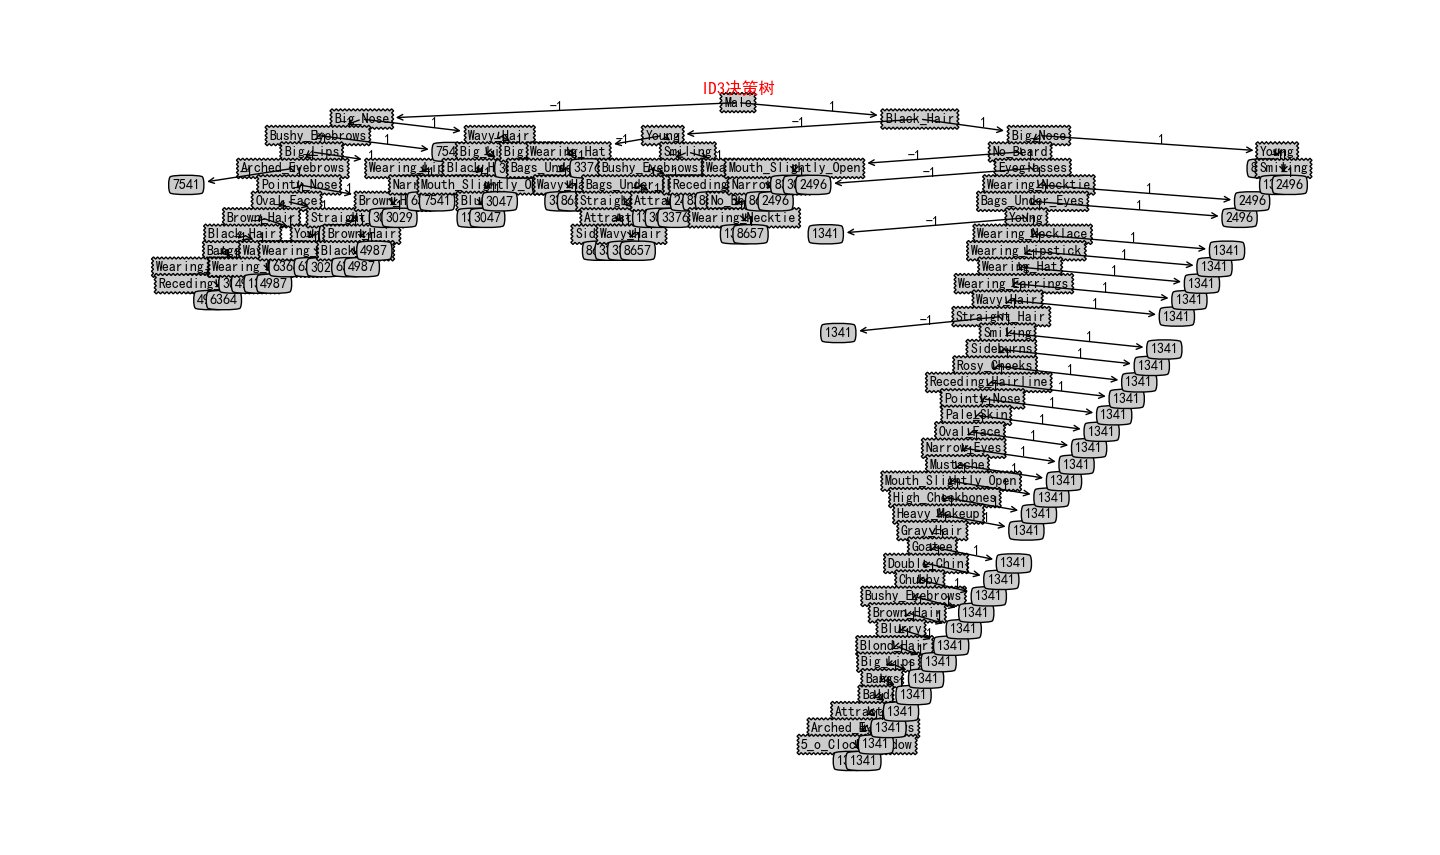
\includegraphics[width=0.45\textwidth]{../figs/celeba_id3_post.png}
    }
    \caption{CelebA 数据集上 ID3 决策树结构对比}
    \label{fig:celeba_id3}
\end{figure}

\noindent 特征重要性(信息增益前 5):Male (0.896) > Wearing\_Lipstick (0.764) > Big\_Nose (0.582) > Heavy\_Makeup (0.530) > Arched\_Eyebrows (0.503)。

\subsubsection{C4.5 算法在 CelebA 上的表现}

C4.5 使用信息增益率作为准则,首选特征为 \textbf{Big\_Nose}(增益率 0.589),而非 ID3 选择的 Male 特征(增益率约 0.9)。\textbf{预剪枝}达到 68\% 准确率,\textbf{后剪枝}达到 84\% 准确率。图 \ref{fig:celeba_c45} 展示了 C4.5 在不同剪枝策略下的决策树结构。

\begin{figure}[H]
    \centering
    \subfloat[C4.5 预剪枝]{
        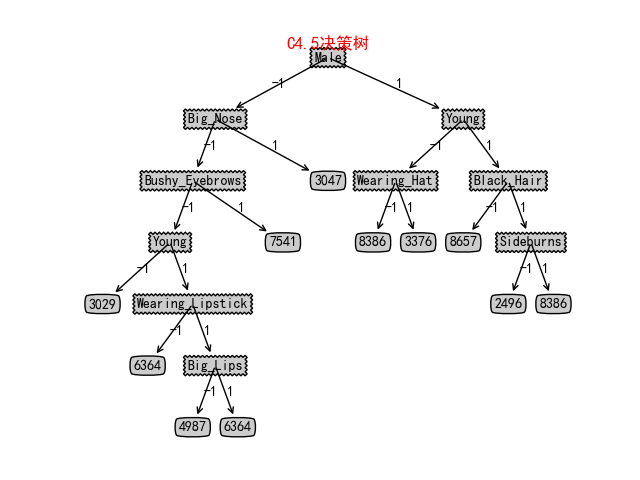
\includegraphics[width=0.45\textwidth]{../figs/celeba_c45_pre.png}
    }
    \hfill
    \subfloat[C4.5 后剪枝]{
        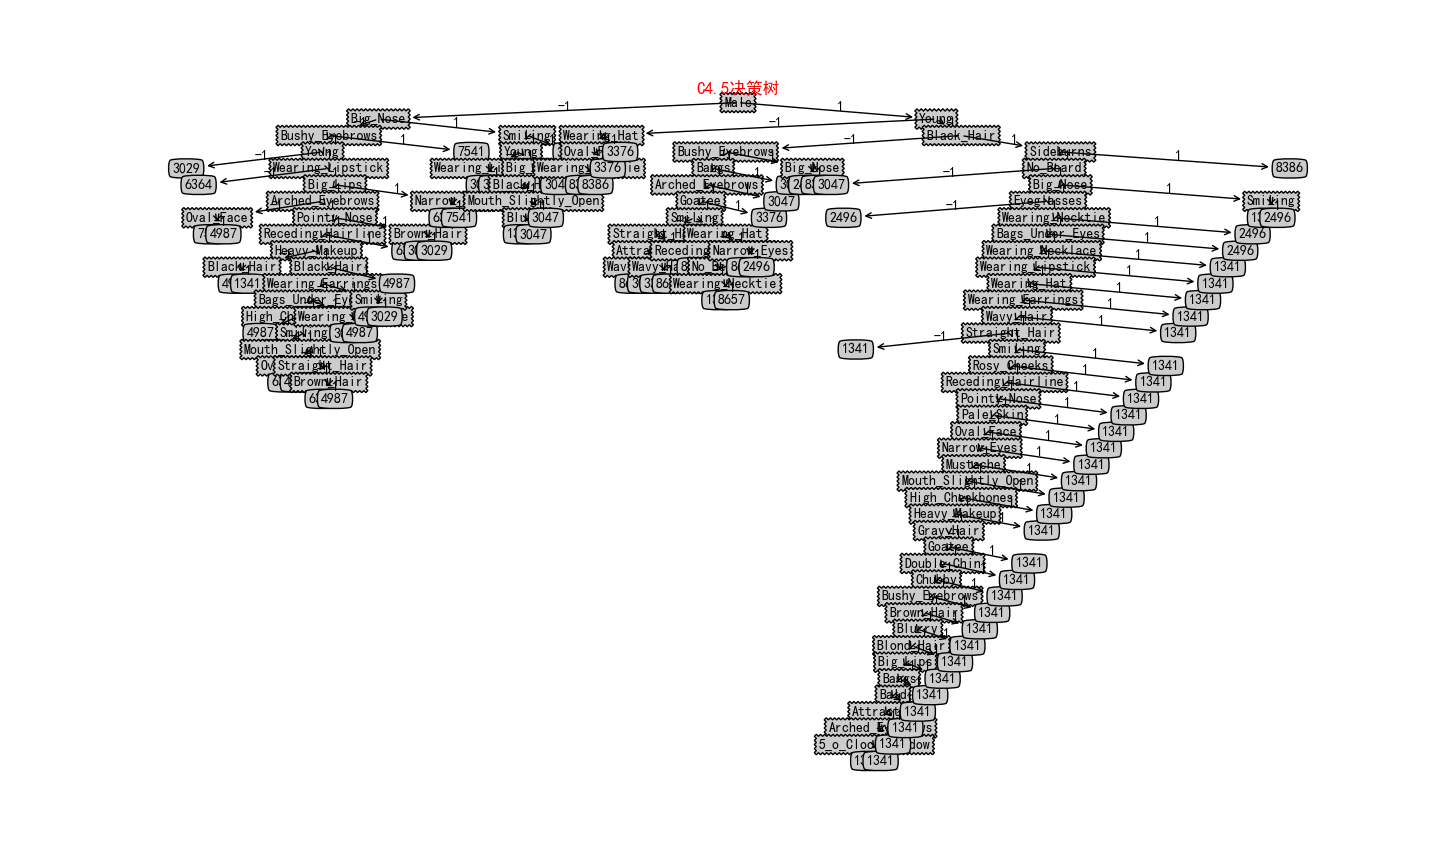
\includegraphics[width=0.45\textwidth]{../figs/celeba_c45_post.png}
    }
    \caption{CelebA 数据集上 C4.5 决策树结构对比}
    \label{fig:celeba_c45}
\end{figure}

\noindent 特征重要性(信息增益率前 5):Big\_Nose (0.589) > Arched\_Eyebrows (0.581) > Goatee (0.511) > Black\_Hair (0.475) > Chubby (0.462)。

\noindent C4.5 的 IV 惩罚了取值分布不均衡的特征,使特征选择更平衡,但在该任务中高判别力的不平衡特征(Male)恰恰最有价值,因此性能略逊于 ID3。

\subsubsection{CART 算法在 CelebA 上的表现}

CART 使用基尼指数作为划分准则,计算效率更高(无需对数运算)。基尼指数公式为 $\text{Gini}(D) = 1 - \sum_{k=1}^{|\mathcal{Y}|}p_k^2$,与信息熵类似但更简洁。CART 首选特征同样为 \textbf{Male}(基尼指数 0.838),与 ID3 一致。\textbf{预剪枝}达到 76\% 准确率,\textbf{后剪枝}达到 84\% 准确率。图 \ref{fig:celeba_cart} 展示了 CART 在不同剪枝策略下的决策树结构。

\begin{figure}[H]
    \centering
    \subfloat[CART 预剪枝]{
        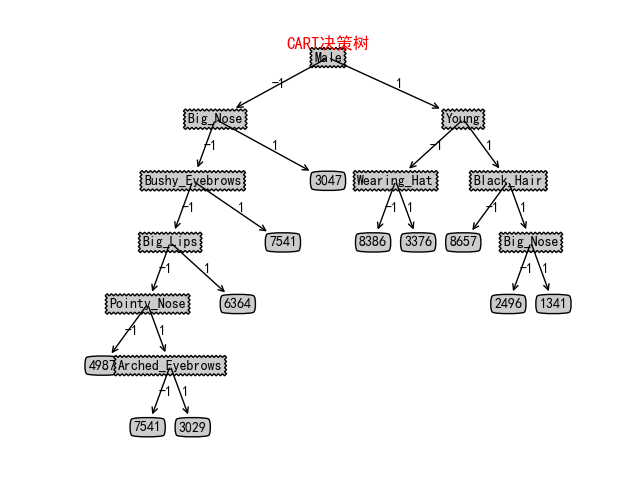
\includegraphics[width=0.45\textwidth]{../figs/celeba_cart_pre.png}
    }
    \hfill
    \subfloat[CART 后剪枝]{
        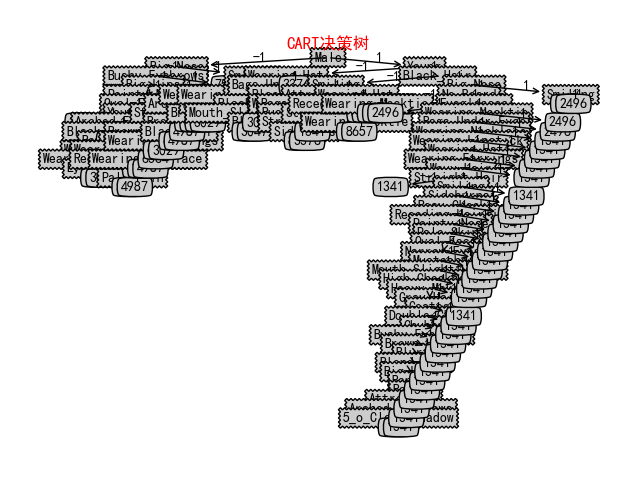
\includegraphics[width=0.45\textwidth]{../figs/celeba_cart_post.png}
    }
    \caption{CelebA 数据集上 CART 决策树结构对比}
    \label{fig:celeba_cart}
\end{figure}

\noindent 特征重要性(基尼指数前 5):Male (0.838) > Big\_Nose (0.853) > Wearing\_Lipstick (0.864) > Arched\_Eyebrows (0.869) > Heavy\_Makeup (0.896,数值越小越重要)。

\noindent CART 的一个重要特点是生成\textbf{二叉树}结构,而 ID3 和 C4.5 生成多叉树。CART 与 ID3 在特征选择上高度一致(均选 Male),性能相当(预剪枝均 76\%,后剪枝分别 84\% vs 86\%),证明了基尼指数与信息增益在实际问题上的等价性。

\section{算法对比与分析}

\subsection{三种算法对比}

\begin{table}[H]
    \centering
    \caption{ID3、C4.5、CART 算法对比}
    \begin{tabular}{lccc}
    \toprule
    \textbf{特性} & \textbf{ID3} & \textbf{C4.5} & \textbf{CART} \\
    \midrule
    划分准则 & 信息增益 & 信息增益率 & 基尼指数 \\
    计算复杂度 & 中等 & 高(需计算IV) & 低(无对数) \\
    特征偏好 & 偏好多值特征 & 修正ID3偏好 & 无明显偏好 \\
    树结构 & 多叉树 & 多叉树 & 二叉树 \\
    \midrule
    \textbf{CelebA准确率} & \textbf{86\%}(后剪枝) & 84\%(后剪枝) & 84\%(后剪枝) \\
    \textbf{首选特征} & Male & Big\_Nose & Male \\
    \bottomrule
    \end{tabular}
\end{table}

\noindent \textbf{算法性能分析}:

\begin{itemize}
    \item \textbf{ID3 vs CART}:两者在特征选择上高度一致(均选 Male 为首选特征),性能相近(86\% vs 84\%),这验证了信息增益与基尼指数在分类任务中的\textbf{理论等价性}。基尼指数本质上是信息熵的二阶近似,两者都衡量数据集的不纯度,因此在实际应用中往往得到相似的划分结果。
    
    \item \textbf{C4.5 的特殊性}:C4.5 通过固有值(IV)惩罚取值数目多的特征,选择了 Big\_Nose 而非 Male。虽然 Male 的信息增益最高(0.896),但其取值分布不均衡导致 IV 较大,使信息增益率降低。这种修正在某些场景下能避免过拟合,但在本数据集上,高判别力的不平衡特征(Male)恰恰最有价值,因此 C4.5 性能略逊(84\% vs 86\%)。
    
    \item \textbf{计算效率}:CART 的基尼指数计算最快(仅需平方运算),ID3 次之(需对数),C4.5 最慢(需同时计算信息增益和 IV)。在大规模数据集上,CART 的计算优势更为明显。
\end{itemize}

\subsection{两种剪枝策略对比}

\begin{table}[H]
    \centering
    \caption{预剪枝与后剪枝对比}
    \begin{tabular}{lcc}
    \toprule
    \textbf{特性} & \textbf{预剪枝} & \textbf{后剪枝} \\
    \midrule
    剪枝时机 & 构建中(贪心) & 构建后(全局) \\
    训练速度 & 快 & 慢 \\
    泛化能力 & 较好 & \textbf{更好} \\
    \midrule
    \textbf{Melon} & 71.43\% & 71.43\% \\
    \textbf{CelebA (ID3)} & 76\% & \textbf{86\%} ↑10\% \\
    \textbf{CelebA (C4.5/CART)} & 68\%/76\% & \textbf{84\%} ↑16\% \\
    \bottomrule
    \end{tabular}
\end{table}

\noindent \textbf{剪枝策略分析}:

\begin{itemize}
    \item \textbf{后剪枝的优势}:在大规模复杂数据集(CelebA)上,后剪枝显著优于预剪枝(ID3 提升 10 个百分点,C4.5/CART 提升 16 个百分点)。这是因为后剪枝基于\textbf{完整树结构进行全局优化},能够识别那些单独看无效但组合后有协同效应的特征划分。例如,某个特征在根节点划分时可能无法提升验证集性能,但与其子节点的特征组合后可能产生强判别能力。
    
    \item \textbf{预剪枝的局限}:预剪枝采用贪心策略,在构建过程中一旦某次划分无法提升验证集性能就停止生长,可能过早终止,导致欠拟合。在 CelebA 上,预剪枝的 C4.5 仅达 68\%,显著低于后剪枝的 84\%,证明了这一点。
    
    \item \textbf{小数据集的特殊性}:在 Melon 数据集上,预剪枝和后剪枝性能相同(均 71.43\%),这是因为样本量小(17 个训练样本),决策树深度有限,两种策略的差异不明显。但剪枝仍然关键——不剪枝仅 42.86\%,剪枝后提升 67\%。

\end{itemize}

\section{实验结论}

本实验系统实现并比较了 ID3、C4.5、CART 决策树算法及预剪枝、后剪枝策略,主要结论:

\begin{enumerate}
    \item \textbf{算法性能}:CelebA 数据集上,ID3+后剪枝最优(86\%),C4.5/CART+后剪枝均达 84\%。ID3 简单高效,但偏好多值特征;C4.5 通过 IV 平衡特征选择,但计算较复杂;CART 使用基尼指数作为划分准则,与 ID3 性能接近。
    
    \item \textbf{剪枝效果}:后剪枝在大数据集上显著优于预剪枝(CelebA:ID3 提升 10\%,C4.5/CART 提升 16\%);剪枝有效缓解过拟合(Melon:从 42.86\% 提升至 71.43\%)。
    
    \item \textbf{特征重要性}:CelebA 数据集中,Male(性别)是最强判别特征(信息增益 0.896,基尼指数 0.838),其次是 Wearing\_Lipstick(0.764)和 Big\_Nose(0.582)。
    
\end{enumerate}

\end{document}
